\documentclass[journal]{IEEEtran}

\usepackage{graphicx}
\usepackage{amsmath}
\usepackage{booktabs}
\usepackage{url}
\usepackage{cite}

\title{Simulation-Based Implementation of Lean Manufacturing Techniques for Productivity Improvement: A Data-Driven Case Study From a Beverage Bottling Line}

\author{
    Your Name,~\IEEEmembership{Student Member, IEEE}
    \thanks{Your Name is with the Department of Production and Industrial Engineering, Your University, Your City, India. Replace this line with your actual affiliation before submission.}
}

\begin{document}

\maketitle

\begin{abstract}
Lean manufacturing is widely recognized as an effective approach for reducing waste and improving productivity, yet many small and medium-sized manufacturing firms struggle to identify which lean techniques will deliver the greatest benefit before implementation. This study develops a data-driven simulation framework to evaluate lean interventions using a real industrial production dataset from a beverage bottling line monitored through an Industrial Internet of Things (IIoT) system. The dataset contains 59 production records across 56 calendar days between July 22, 2022 and February 6, 2023, 265 hourly operating observations, and 1,388 downtime events. First, the operational profile of the line is analyzed through production, efficiency, and downtime metrics. Next, an event-level bootstrap simulation is used to test three lean scenarios: 5S with visual management, total productive maintenance (TPM), and an integrated lean bundle combining micro-stoppage reduction, minor-stop reduction, and major-stop reduction. The baseline system produced 212,358 liters with an overall availability of 42.66\%. Downtime analysis showed that micro-stoppages represented 61.31\% of all events but only 13.59\% of downtime minutes, while major stoppages represented only 6.77\% of events but 66.26\% of downtime minutes. Simulation results indicate that 5S and visual management yield a modest output gain of 2.33\%, TPM yields 20.61\%, and the integrated lean bundle yields 32.19\%, while increasing simulated availability from 42.37\% to 55.33\%. The results show that, for this line, reducing major downtime events produces much greater productivity gains than focusing only on frequent short interruptions. The study contributes a reproducible open-data approach for simulation-based lean evaluation and offers a practical roadmap for SME-oriented manufacturing improvement.
\end{abstract}

\begin{IEEEkeywords}
Lean manufacturing, discrete-event simulation, productivity improvement, SMEs, bottling line, downtime analysis, total productive maintenance, 5S, IIoT, digital manufacturing.
\end{IEEEkeywords}

\section{Introduction} 
Lean manufacturing has become a major operational strategy for improving throughput, reducing waste, and increasing process stability across manufacturing sectors \cite{belekoukias2014lean}. However, implementation remains difficult in small and medium-sized enterprises (SMEs), where firms often face tight budgets, limited analytical capability, and little tolerance for failed improvement projects. In such settings, simulation provides a practical way to test lean alternatives before modifying the actual shop floor \cite{yu2021sme, frecassetti2023italian}.

Recent literature shows that lean tools can improve operational performance, but their impact is strongly context dependent \cite{belekoukias2014lean, possik2022lean}. Some studies demonstrate that simulation can identify which lean practices provide the greatest benefit in a specific system \cite{frecassetti2023italian}. Other work shows that lean and smart manufacturing increasingly reinforce each other, especially when digital production data are available \cite{bokhorst2022smart, reslan2025digital}. Yet the SME simulation literature still highlights the shortage of targeted, reproducible empirical cases \cite{yu2021sme}.

This study addresses that gap by using a real open industrial dataset from a beverage bottling line collected through an IIoT monitoring system \cite{david2026dataset, david2024iot}. Unlike many prior lean-simulation studies built on proprietary case-company data, the present work uses public event-level downtime data and transparent scenario assumptions. The objective is to evaluate how different lean interventions may improve productivity under real operational variability.

The contributions of the paper are threefold:
\begin{enumerate}
    \item it characterizes the production and downtime behavior of a real bottling line;
    \item it identifies the dominant waste pattern through downtime-event analysis; and
    \item it provides a reproducible simulation framework for prioritizing lean interventions in SME-relevant manufacturing systems.
\end{enumerate}

\section{Literature Review}
Lean manufacturing is well established as an approach for improving operational performance through waste reduction, process discipline, and flow improvement \cite{belekoukias2014lean}. However, organizations often struggle to determine which tools should be prioritized first. Possik \emph{et al.} \cite{possik2022lean} showed through co-simulation that some lean tools such as 5S may be broadly useful, while others such as SMED or cross-training are more context sensitive. Frecassetti \emph{et al.} \cite{frecassetti2023italian} demonstrated in an Italian SME that simulation can support the selection of lean practices by quantifying their effect before implementation.

Simulation is particularly valuable for SMEs because it reduces trial-and-error implementation risk. Yu and Chen \cite{yu2021sme} reviewed factory simulation in SMEs and concluded that adoption barriers remain substantial, especially around expertise, cost, and transferability. Oleghe and Salonitis \cite{oleghe2019hybrid} further argued that lean modeling still needs stronger quantitative treatment, especially where process behavior is dynamic and uncertain.

The literature also shows increasing convergence between lean and digital manufacturing. Bokhorst \emph{et al.} \cite{bokhorst2022smart} found that smart manufacturing usually builds on lean principles rather than replacing them. Reslan \emph{et al.} \cite{reslan2025digital} reported that digital-twin-enabled value stream mapping can strengthen lean diagnosis with real-time data. In the food and beverage context, Matindana and Shoshiwa \cite{matindana2025tanzania} showed that lean implementation remains highly relevant for SMEs, but quantitative simulation-oriented evidence is still limited.

Based on this literature, the main research gap is clear: most lean-simulation studies remain case-specific and proprietary, while very few combine real event-level production data, downtime logs, and simulation-based evaluation of lean scenarios in SME-relevant manufacturing settings. This paper responds to that gap using an open industrial dataset and a reproducible simulation workflow.

\section{Problem Formulation and Performance Measures}
The key production and availability relationships used in the study are given below.

\subsection{Operational Availability}
\begin{equation}
A = \frac{T_{op}}{T_{mon}}
\end{equation}
where $A$ is operational availability, $T_{op}$ is effective operating time, and $T_{mon}$ is monitored time.

\subsection{Downtime}
\begin{equation}
T_{dt} = T_{mon} - T_{op}
\end{equation}
where $T_{dt}$ is downtime or pause time.

\subsection{Production Rate}
\begin{equation}
R = \frac{Q}{T_{op}}
\end{equation}
where $R$ is production rate in liters per operating hour and $Q$ is liters produced.

\subsection{Scenario-Based Output}
\begin{equation}
Q' = R \times (T_{mon} - T'_{dt})
\end{equation}
where $Q'$ is simulated output under an improvement scenario and $T'_{dt}$ is the scenario-adjusted downtime.

\subsection{Downtime Transformation}
\begin{equation}
T'_{dt} = T_{res} + \sum_{i=1}^{n}\alpha_i t_i
\end{equation}
where $T_{res}$ is residual downtime not represented at event level, $t_i$ is the duration of downtime event $i$, and $\alpha_i$ is the improvement factor for that downtime category.

\subsection{Productivity Improvement}
\begin{equation}
\%\Delta Q = \frac{Q' - Q}{Q}\times 100
\end{equation}

\section{Research Methodology}
\subsection{Dataset}
The study uses the open dataset \emph{Industrial Production Time-Series Dataset from a Beverage Bottling Line}, published on Zenodo on January 4, 2026 \cite{david2026dataset}. The data were collected from a real industrial filling machine using an IIoT monitoring system with sensor-based production counting and downtime logging. The monitoring period covers July 22, 2022 to February 6, 2023.

The dataset contains:
\begin{itemize}
    \item 59 production summary records,
    \item 56 calendar production days,
    \item 265 hourly operating observations, and
    \item 1,388 downtime events.
\end{itemize}

\subsection{Research Design}
The research follows a data-driven simulation case-study approach:
\begin{enumerate}
    \item baseline analysis of production and downtime behavior;
    \item classification of downtime into lean-relevant categories;
    \item definition of lean scenarios based on literature and operational logic; and
    \item bootstrap simulation of counterfactual performance.
\end{enumerate}

\subsection{Baseline Analysis}
The variables used in the analysis were liters produced, production units, monitored time, operation time, pause time, hourly efficiency, downtime-event duration, and product type (3 L and 5 L). Downtime events were grouped into three categories:
\begin{itemize}
    \item micro-stoppages: $t \leq 2$ minutes,
    \item minor stoppages: $2 < t \leq 10$ minutes,
    \item major stoppages: $t > 10$ minutes.
\end{itemize}

\subsection{Simulation Logic}
An event-level bootstrap simulation with 5,000 replications was developed from the observed day profiles. Each replication resampled observed production days with replacement, preserving real variability in monitored time, production rate, and downtime structure. Event durations were normalized to recorded daily pause time so that the simulated baseline remained aligned with the plant record.

Three improvement scenarios were tested:
\begin{enumerate}
    \item \textbf{5S + Visual Management:} 15\% of micro-stoppages eliminated;
    \item \textbf{TPM:} major stoppage durations reduced by 25\%;
    \item \textbf{Integrated Lean Bundle:} 20\% of micro-stoppages eliminated, minor stoppages reduced by 15\%, and major stoppages reduced by 30\%.
\end{enumerate}

These scenario values are literature-informed assumptions intended for comparative evaluation. They should not be interpreted as guaranteed post-implementation outcomes.

\section{Results}
\subsection{Baseline Operational Performance}
The line produced 212,358 liters from 60,888 units during 238.65 monitored hours. Effective operating time was 101.81 hours and downtime was 137.56 hours, giving an overall availability of 42.66\%. The mean daily efficiency from the summary records was 46.52\%.

The 3 L product had an average production rate of 1,963.71 L/h, while the 5 L product averaged 2,918.68 L/h. At the date-aggregated level, pause time showed a strong negative correlation with efficiency ($r=-0.707$), indicating that downtime is a dominant productivity driver.

\begin{table}[!t]
\caption{Baseline Performance Indicators}
\label{tab:baseline}
\centering
\begin{tabular}{lr}
\toprule
Metric & Value \\
\midrule
Production days & 56 \\
Production summary records & 59 \\
Hourly observations & 265 \\
Downtime events & 1,388 \\
Total production & 212,358 L \\
Total units produced & 60,888 \\
Monitored time & 238.65 h \\
Operating time & 101.81 h \\
Pause time & 137.56 h \\
Overall availability & 42.66\% \\
\bottomrule
\end{tabular}
\end{table}

\subsection{Downtime Structure}
The downtime pattern is highly skewed. The median downtime event was 1.50 minutes, the 90th percentile was 6.50 minutes, the 95th percentile was 13.74 minutes, and the maximum event lasted 349.83 minutes. Micro-stoppages accounted for 851 events, minor stoppages for 443 events, and major stoppages for 94 events.

Although major stoppages represented only 6.77\% of events, they consumed 66.26\% of total downtime minutes. By contrast, micro-stoppages represented 61.31\% of events but only 13.59\% of downtime minutes. This finding suggests that event frequency alone is a poor basis for lean-priority selection.

\begin{figure}[!t]
\centering
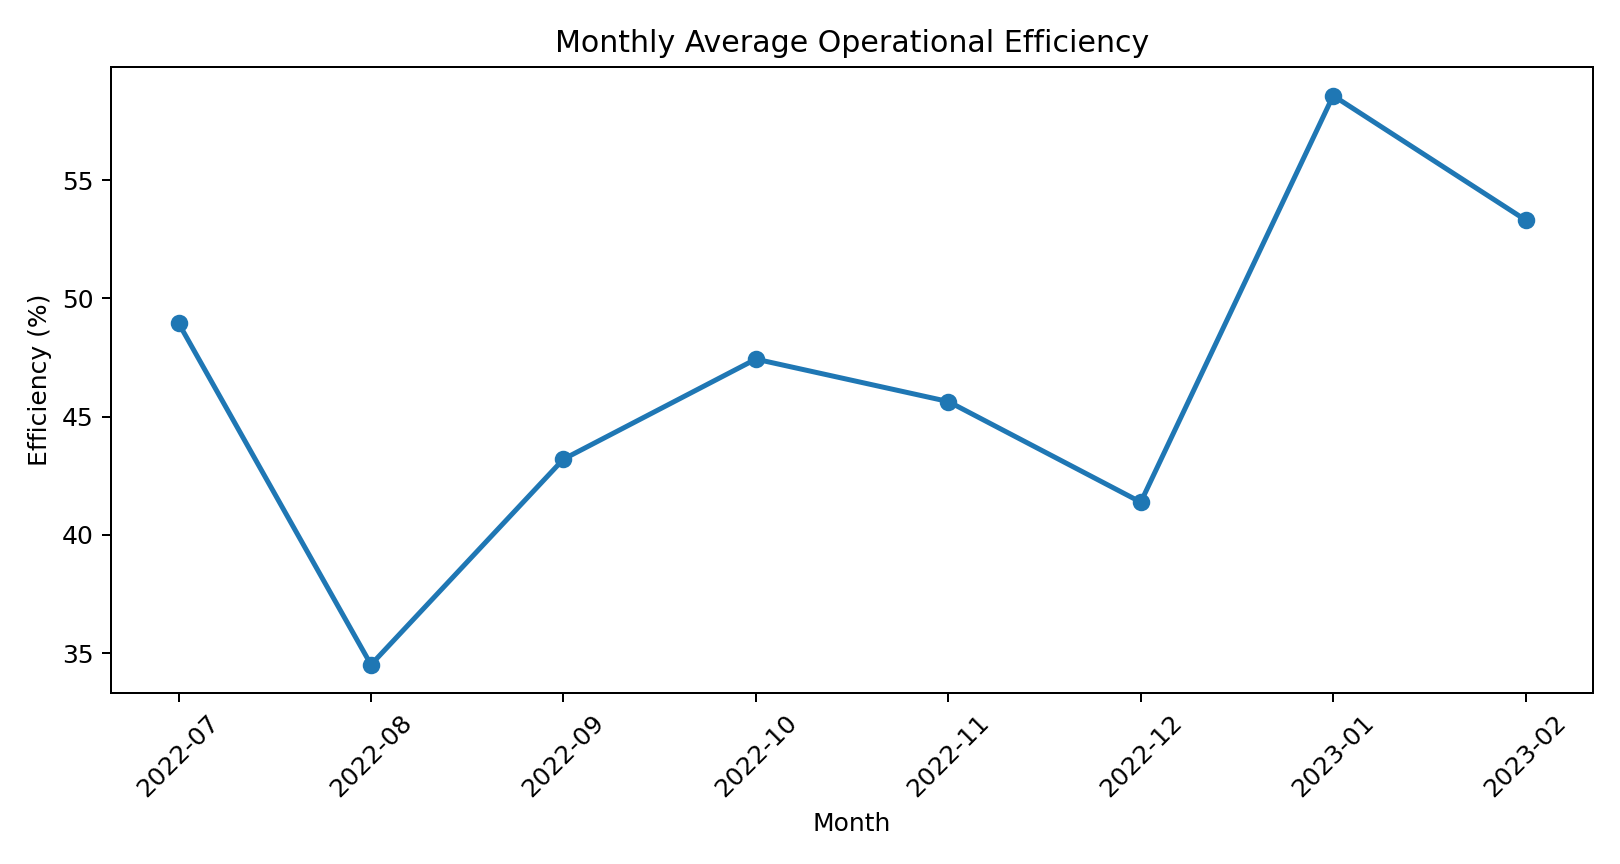
\includegraphics[width=\columnwidth]{outputs/monthly_efficiency.png}
\caption{Monthly average operational efficiency for the bottling line.}
\label{fig:monthly}
\end{figure}

\begin{figure}[!t]
\centering
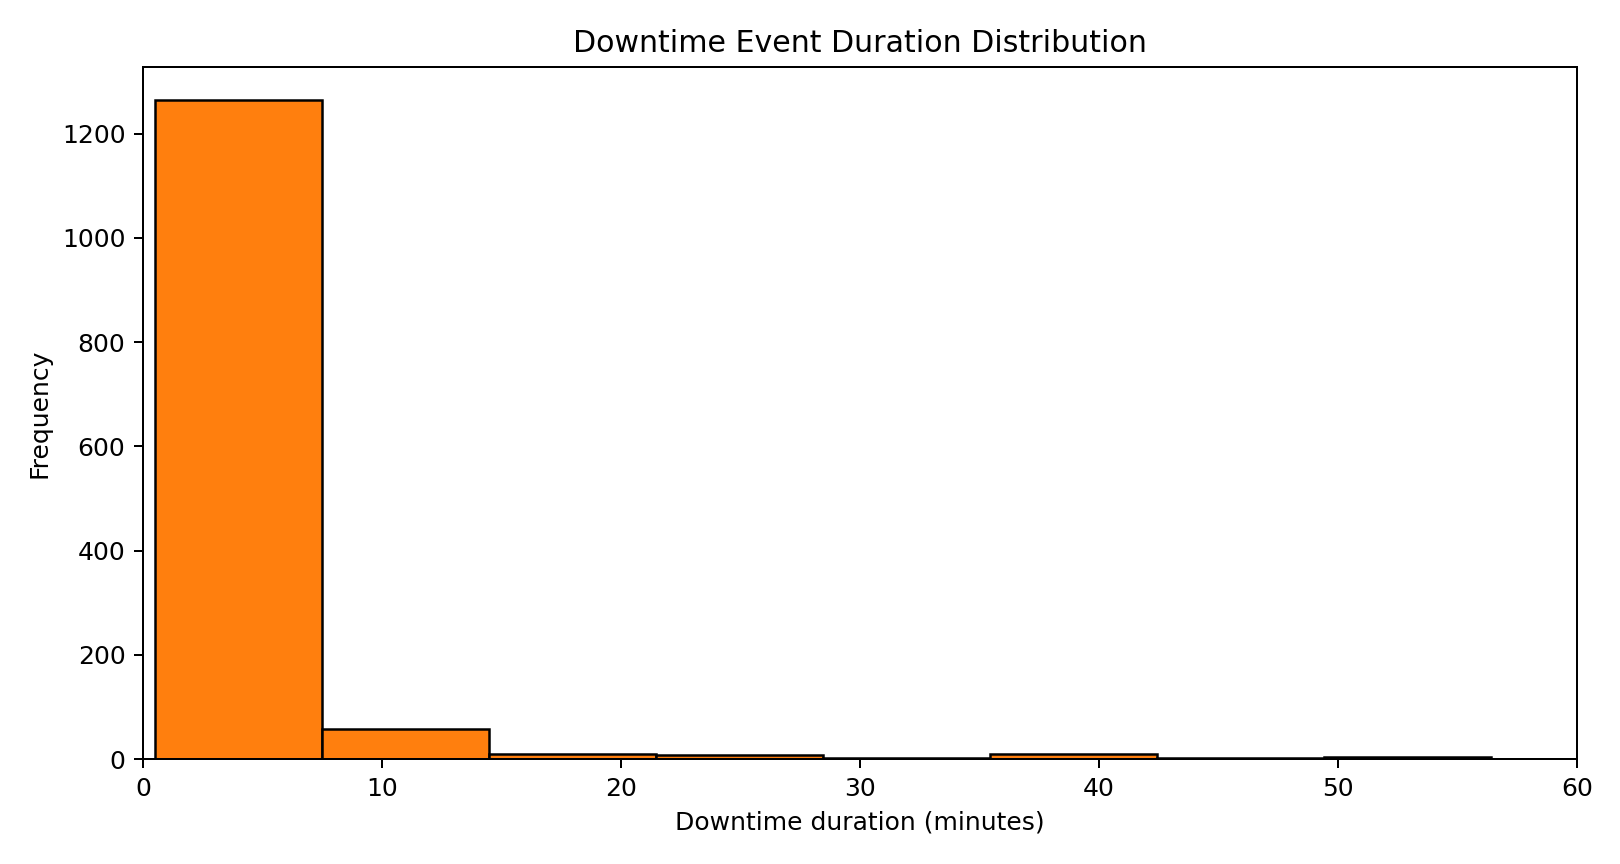
\includegraphics[width=\columnwidth]{outputs/downtime_distribution.png}
\caption{Distribution of downtime-event duration, truncated at 60 minutes for readability.}
\label{fig:downtime}
\end{figure}

\subsection{Simulation Results}
Table~\ref{tab:scenario} summarizes the counterfactual results. The simulated baseline produced 211,924.69 liters on average across the resampled production horizon, closely matching the observed system output.

\begin{table}[!t]
\caption{Simulation Results for Lean Scenarios}
\label{tab:scenario}
\centering
\begin{tabular}{lrrrr}
\toprule
Scenario & Output (L) & Gain (\%) & Eff. (\%) & Eff. Gain (pp) \\
\midrule
Baseline & 211,924.69 & 0.00 & 42.37 & 0.00 \\
5S + Visual Mgmt. & 216,866.69 & 2.33 & 43.25 & 0.88 \\
TPM & 255,604.10 & 20.61 & 50.81 & 8.44 \\
Integrated Lean Bundle & 280,142.22 & 32.19 & 55.33 & 12.96 \\
\bottomrule
\end{tabular}
\end{table}

The integrated lean bundle produced the largest improvement, increasing mean output by 68,217.53 liters compared with the simulated baseline. However, the most important managerial insight is that TPM alone delivered much stronger gains than 5S alone. This occurs because major stoppages dominate lost time in this system.

\begin{figure}[!t]
\centering
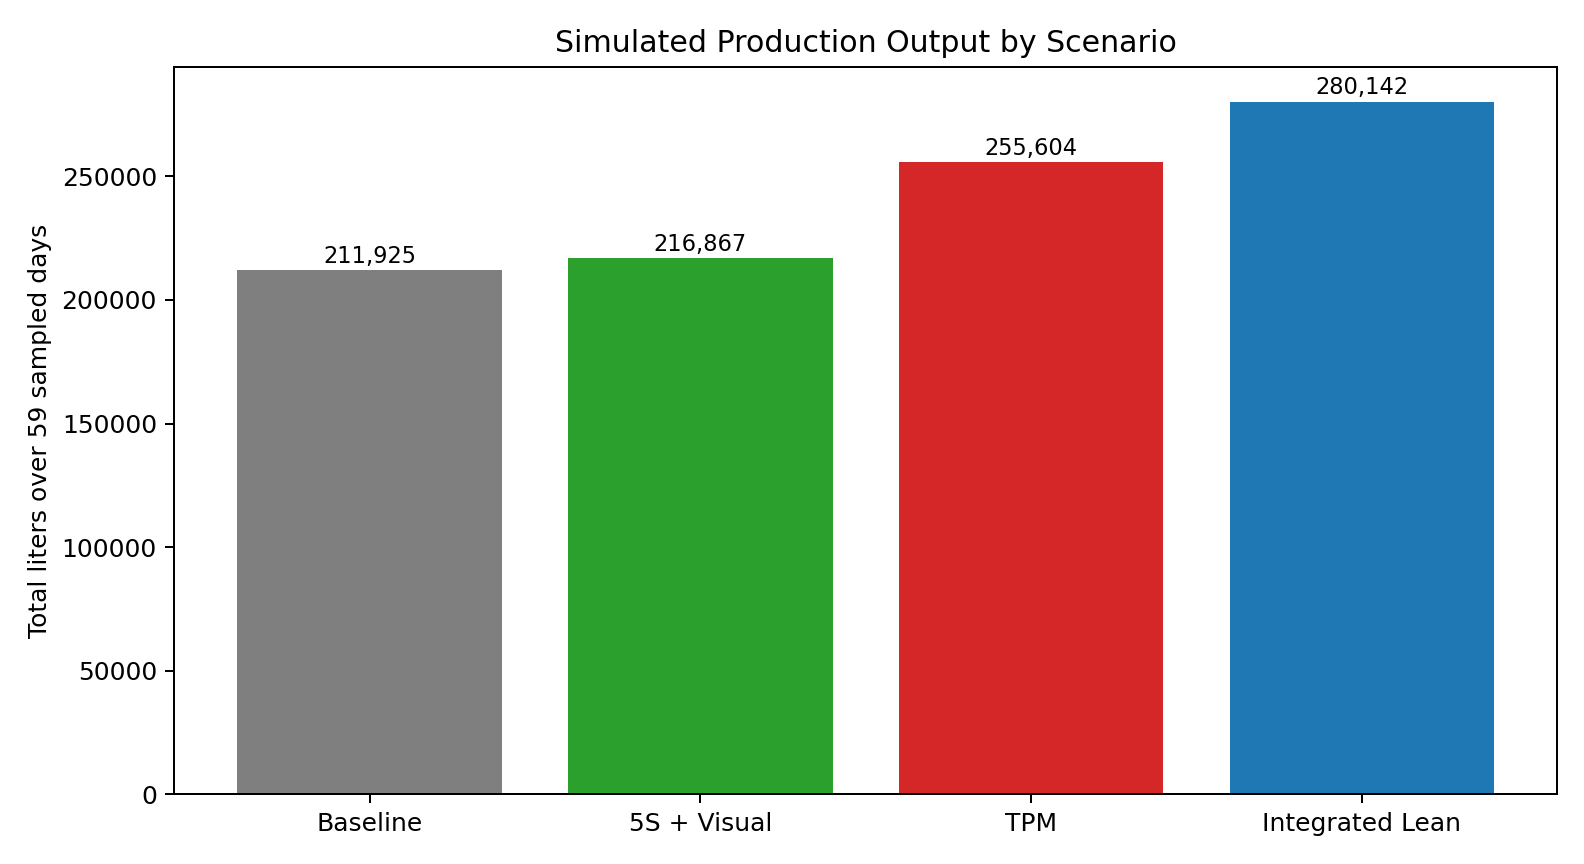
\includegraphics[width=\columnwidth]{outputs/scenario_output.png}
\caption{Mean simulated production output across the baseline and lean scenarios.}
\label{fig:scenario}
\end{figure}

\section{Discussion}
Three findings stand out. First, lean priorities should be aligned with downtime severity rather than event frequency alone. If managers focus only on frequent short interruptions, they may overinvest in micro-stop reduction while neglecting a small number of long stoppages that dominate lost time.

Second, 5S and visual management still have value, but their contribution is incremental in this case. The simulation suggests that workplace organization and visual control can improve flow stability, yet they do not address the primary source of productivity loss by themselves. This is consistent with earlier work showing that some lean tools are broadly beneficial, whereas others should be chosen according to system context \cite{possik2022lean, frecassetti2023italian}.

Third, the study illustrates the value of integrating lean thinking with digital production data. Prior work on smart manufacturing and digital value stream mapping suggests that real-time data can strengthen lean decision-making \cite{bokhorst2022smart, reslan2025digital}. The present results support that claim: event-level downtime records make it possible to quantify which intervention should be prioritized first, rather than relying only on observation or expert opinion.

For SME-oriented industries, this matters because firms often cannot afford multiple failed improvement projects. A simulation-first approach can reduce implementation risk by screening alternatives before physical deployment.

\section{Conclusion}
This paper developed a simulation-based framework for evaluating lean manufacturing interventions using a real industrial bottling-line dataset. The baseline analysis showed low availability, high downtime, and strong variability in production performance. Although micro-stoppages were the most frequent events, major stoppages dominated total downtime.

The simulation indicates that 5S and visual management produce a modest gain of 2.33\%, TPM produces a much stronger gain of 20.61\%, and an integrated lean bundle increases output by 32.19\% while raising mean simulated availability from 42.37\% to 55.33\%.

The main managerial implication is that maintenance-led reduction of major stoppages should be prioritized first for this bottling line, followed by broader stabilization practices such as 5S, standardized work, and visual management. The main research contribution is methodological: the paper presents a transparent and reproducible open-data framework for simulation-based lean analysis that can be adapted by students, researchers, and SME practitioners.

\section*{Limitations and Future Work}
The lean interventions were simulated as literature-informed scenarios rather than validated post-implementation plant outcomes. In addition, the dataset does not provide root-cause labels for downtime events, so the mapping from downtime category to lean tool remains inferential. Future work can extend the model by collecting cause-coded downtime data, labor variables, and quality-loss records, then validating the proposed interventions through a real shop-floor pilot.

\bibliographystyle{IEEEtran}
\bibliography{references}

\end{document}
